\chapter{Memory-device implication: 알고리즘 이름보다 workload primitive}
\label{STC-S14}

Memory-device 회사의 기회는 ``per-user weight sleep이 주류가 된다''는 한 시나리오에 종속되어서는 안
된다. External dominant, hybrid, periodic refresh, niche, broad adoption 모두에서 살아남는 traffic과
control primitive를 먼저 찾는다. 이 장은 market size나 제품 우위를 주장하지 않고, 측정해야 할
workload를 도출한다.

\begin{cautionbox}[Patent-first publication boundary]
Veridraft는 device 제품화에 관한 10개 P3 hypothesis를 internal/patent-first hold로 분류했다. 따라서
공개 claim ledger에는 해당 문장과 구현 세부를 싣지 않는다. 아래 내용은 이미 공개된 source에서 도출한
workload class와 evaluation question이며, 특정 제품 architecture나 권리 주장을 승인하는 문서가 아니다.
상세 opportunity matrix는 별도 내부 review를 거쳐야 한다.
\end{cautionbox}

\section{왜 inference memory와 다른 trace가 생기는가}

Fixed-model inference는 큰 weight의 read-mostly access, KV append/read, activation traffic이 중심이다.
Wake--sleep memory system은 여기에 네 종류를 추가한다.

\begin{enumerate}
  \item \textbf{Version traffic}: candidate, predecessor, snapshot, rollback reserve가 동시에 존재한다.
  \item \textbf{Index mutation}: vector payload, embedding key, graph edge, temporal validity가 함께 바뀐다.
  \item \textbf{Small-artifact fan-out}: user/cohort adapter, router catalog, recurrent state가 많아지고 hot set이
  시간에 따라 바뀐다.
  \item \textbf{Lineage control}: source handle, parent/replacement edge, delete epoch, validation attestation을
  low-tail-latency로 조회한다.
\end{enumerate}

따라서 peak bandwidth만 높인 장치보다 capacity, endurance, random metadata latency, copy-on-write,
atomic generation change, encryption domain, rebuild throughput의 조합이 중요해진다.

\begin{figure}[htbp]
  \centering
  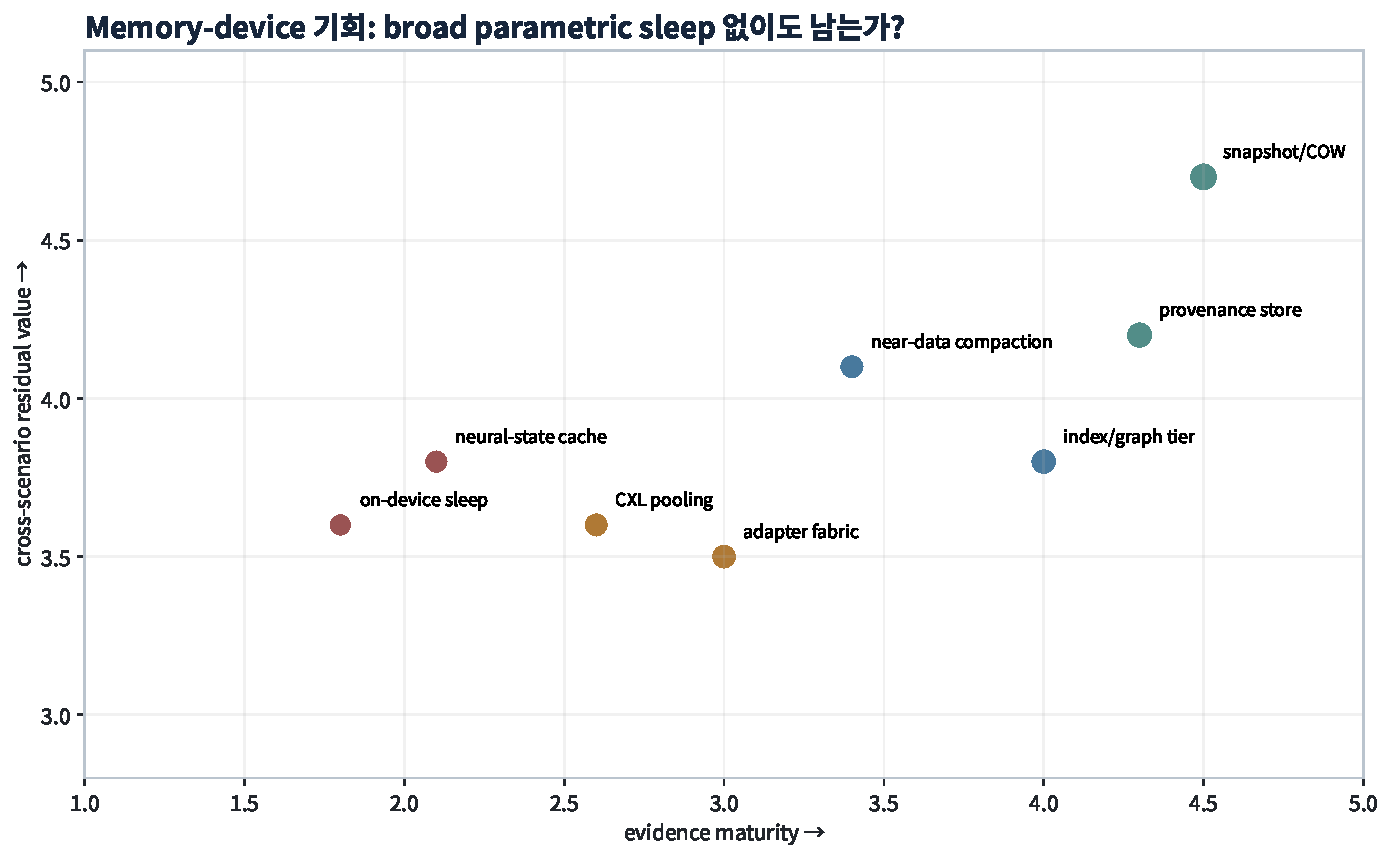
\includegraphics[width=0.97\textwidth]{figures/stc-f012.pdf}
  \caption{공개 source에서 관찰 가능한 workload class를 evidence maturity와 cross-scenario residual
  value의 두 축에 배치한 research map. 좌표는 제품 추천이나 시장 예측이 아니라 benchmark 우선순위를
  정하기 위한 정성적 가설이다.}
  \stcfigure{STC-F012}
  \figsource{Original research map; SRC-STC-0056, SRC-STC-0065}{Snapshot, provenance, mutable index, state cache, pooling, local compaction 등 workload 후보를 두 축에 놓은 산점도.}
  \label{fig:device-research-map}
\end{figure}

\section{Cross-scenario workload classes}

\begin{longtable}{L{0.18\textwidth} L{0.25\textwidth} L{0.22\textwidth} L{0.20\textwidth}}
\caption{Device 연구가 먼저 계측할 workload primitive}\label{tab:device-primitives}\\
\toprule
Class & Trace primitive & 시스템 가치 질문 & 비-STC residual value \\
\midrule
\endfirsthead
\toprule
Class & Trace primitive & 시스템 가치 질문 & 비-STC residual value \\
\midrule
\endhead
provenance episode & append, scan, sparse delete, lineage traversal & rebuild 범위와 audit latency를 줄이는가 & temporal RAG에도 높음 \\
snapshot/version & COW clone, multi-object publish, predecessor pin & rollback peak bytes/RTO를 줄이는가 & model/index release에도 높음 \\
mutable index/graph & small random rewrite, compaction, re-embed & write amplification과 tail latency는 얼마인가 & agent memory 전반에 높음 \\
state cache & recurrent/KV/adapter load, compatibility lookup & token prefix 외 state reuse를 회복하는가 & RNN/neural memory serving에 높음 \\
tiered pool & HBM--DRAM--CXL--storage migration & base duplicate와 state movement를 동시에 줄이는가 & inference와 refresh에도 높음 \\
local preprocessing & dedup, cluster, filter, graph maintenance & 이동 bytes/energy 절감이 local compute penalty보다 큰가 & data pipeline에도 중간--높음 \\
on-device idle work & burst train/compact, thermal pause, checkpoint & privacy benefit이 battery/endurance를 상쇄하는가 & local personalization에 높음 \\
lifecycle telemetry & per-item bytes, age, reuse, rollback, erase & useful retained evidence를 측정할 수 있는가 & 모든 memory system에 높음 \\
\bottomrule
\end{longtable}

\section{장치 요구사항을 metric으로 번역하기}

\textbf{Capacity.} Live state만이 아니라 candidate, pinned predecessor, migration duplicate, workspace,
replica를 포함한 $B_{peak,physical}(t)$를 측정한다. Snapshot 기능이 있어도 logical clone과 physical
dirty-page growth를 분리한다.

\textbf{Endurance.} Host write bytes뿐 아니라 device-level write amplification을 index/graph rewrite,
compaction, garbage collection, secure reclamation별로 분해한다. Update frequency가 서로 다른 CMS 또는
adapter tier는 한 평균 write rate로 합치지 않는다.

\textbf{Bandwidth와 locality.} Sequential episode scan, random ANN/graph access, checkpoint delta,
adapter page-in, validation readback을 각각 측정한다. Near-data operator는 saved link bytes와 추가 local
execution, model residency, result validation cost를 함께 보고한다.

\textbf{Tail latency.} Manifest, compatibility, lineage, deny-root lookup은 작은 I/O지만 wake request의
critical path에 있다. Bulk GB/s가 높아도 P99 metadata lookup이 길면 serving head를 안전하게 pin할 수
없다.

\textbf{Security와 recovery.} Tenant key boundary, instant deny, physical erase, stale replica discovery,
rollback-after-delete를 fault injection한다. Encryption throughput만으로 derived-state deletion을
증명하지 않는다.

\section{Device--system 공동 DSE}

하드웨어 design space exploration의 입력은 다음과 같이 workload에서 직접 온다.

\begin{equation}
\mathcal D=\{B_{source},B_{base},B_{delta},B_{index},B_{recovery},
R/W\ pattern,\tau_{cadence},Q_{age},R_v,\text{privacy locality}\}.
\end{equation}

출력은 later-wake utility floor 아래에서 total energy, bytes moved, write amplification, physical peak,
P99 wake interference, sleep completion age, rollback/delete time의 Pareto frontier다. 특정 장치가 sleep
job을 빨리 끝냈어도 base replica나 migration이 전체 비용을 키우면 system win이 아니다.

\section{의사결정 순서}

\begin{enumerate}
  \item 공개 trace와 simulator로 primitive를 먼저 검증한다.
  \item External-only와 periodic-refresh에도 가치가 남는 기능을 Tier 1으로 둔다.
  \item Hybrid/broad scenario에만 가치가 큰 state/adapter 기능은 leading indicator를 조건으로 둔다.
  \item Patentability, freedom-to-operate, security review가 끝나기 전에는 public claim으로 승격하지 않는다.
  \item 제품 KPI를 bandwidth가 아니라 useful retained evidence per lifecycle resource로 연결한다.
\end{enumerate}

\begin{keypoint}[Device 관점의 핵심]
가장 강건한 기회는 ``sleep training 전용 memory''라는 이름이 아니라, versioned derived state를 많이
만들고 검증하고 되돌리는 시스템의 memory primitive다. Parametric sleep이 지연되어도 provenance,
snapshot, temporal index, heterogeneous state caching과 lifecycle telemetry workload는 남는다.
\end{keypoint}
